\documentclass[a4paper,11pt]{report}

\usepackage[utf8]{inputenc}
\usepackage[T1]{fontenc}
\usepackage[francais]{babel}

\usepackage{graphicx}
\usepackage{tabularx}
\usepackage{arydshln}

\usepackage{pdflscape}
\usepackage{pdfpages}
\usepackage{chronology}
%%%%%%%%%%%%%% http://tex.stackexchange.com/questions/171782/error-with-chronology-and-babel-packages-paragraph-ended-before-pgffornex %%%%%%%%%%%%%%
\let\CHRONOLOGY\chronology
\let\endCHRONOLOGY\endchronology
\def\chronology{\shorthandoff{;}\CHRONOLOGY}
\def\endchronology{\endCHRONOLOGY\shorthandon{;}}
%%%%%%%%%%%%%%%%%%%%%%%%%%%%%%%%%%%%%%%%%%%%%%%%%%%%%%%%
\usepackage{fullpage}
\usepackage{hyperref}

\setcounter{secnumdepth}{3}

\title{Evalens -- Analyse}
\date{}

\begin{document}
\maketitle
\tableofcontents

\chapter{Lexique}

\subsection{Doyen}

\subsection{Gestionnaire de campagne}
S'occupe de la gestion d'une camapagne d'évaluation.
Entité pouvant être composée de plusieurs personnes.

\subsection{Superviseur}

\subsection{Gestionnaire de communication}
Transversal aux facultés.

\subsection{Chargé de communication facultaire}
Communique différentes informations relatives aux campagnes d'évaluations à la communauté universitaire.

\subsection{Gestionnaire pédagogique faculaire}
Toute personne ayant une responsabilité au niveau faculaire dans le traitement des résultats de campagne, la consultation de ces résultats et la gestion des questionnaires de campagne.

\subsection{Commision pédagogique facultaire}
cd. règlement cadre.
\subsubsection{Membre}
\subsubsection{Président}
Le président siège au conseil des commissions pédagogiques.

\subsection{Conseil des commissions pédagogiques (CoCoPe)}
Conférence rassemblant les présidents et vice-présidents de chaque commission pédagogique facultaire, ainsi que le recteur, vice-recteur à l'enseignement et deux conseillers pédagogiques désignés par ces derniers.
Ce conseil est présidé par le recteur ou le vice-recteur qu'il désigne.

Le CoCoPe a le pouvoir de modifier le règlement cadre et a pour tâche de mettre à jour la banque de questionnaires.

% \subsection{CoA}

\subsection{Unité d'enseignement}

\subsection{Étudiant}
Personne inscrite régulièrement à l'Université Libre de Bruxelles et suivant un certain nombre d'unités d'enseignement.

\subsection{Enseignant}
Personne dispensant une unité d'enseignement à un ensemble d'étudiants.
Il peut s'agir d'un professeur ou d'un assitant, titulaire ou non de chacune des unités d'enseignement auxquelles il participe.

\subsection{Titulaire}
Un enseignant est titulaire d'une unité d'enseignement s'il en est l'enseignant principal.
Ce statut lui donne accès aux évaluations des enseignants non-titulaires pour les unités d'enseignement qu'ils ont en commun.

\subsection{Cellule de communication universitaire}

\subsection{Campagne d'évaluation}


\subsection{Enquête}
Processus regroupant la prise d'avis des étudiants, le traitement des résultats ainsi que la consultation de ces derniers.

\subsection{Calendrier}
Ensemble de dates et de périodes liées à une campagne d'évaluation.

\subsection{Période}
Intervalle de temps ayant une date et une heure de début et de fin.

\subsection{Département de support aux activités académiques (DSAA)}

\subsection{Directeur administratif facultaire (DAF)}














\chapter{Cas d'utilisation}

\section{Administration}

\begin{figure}[ht]
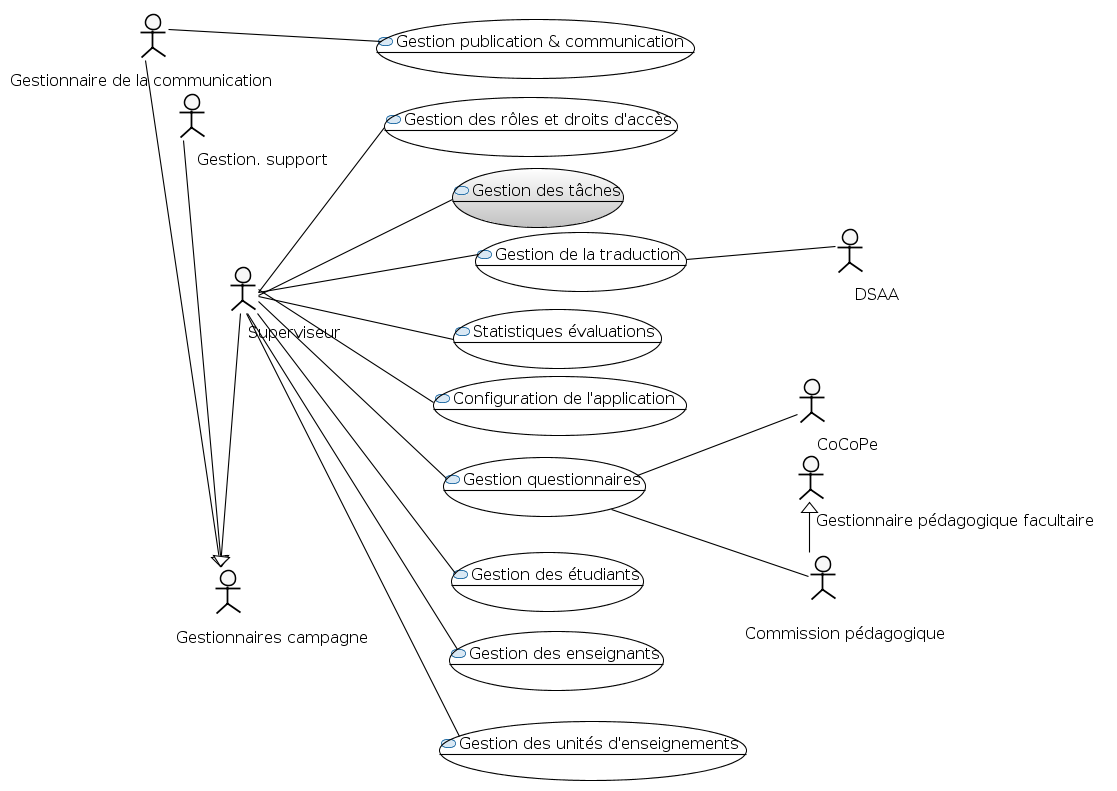
\includegraphics[width=\linewidth]{workspace/evalens-usecases/administration.png}
\caption{Diagramme des cas d'utilisation du système administratif.}
\label{fig:usecase-admin}
\end{figure}


%%%%%%%%%%%%%%%%%%%%%%%%%%%%%%%%%%%%%%%%%%%%%%%%%%%%%%%%%%%%%%%
%      GESTION DES RÔLES ET DES DROITS D'ACCÈS
%%%%%%%%%%%%%%%%%%%%%%%%%%%%%%%%%%%%%%%%%%%%%%%%%%%%%%%%%%%%%%%
\subsection{Gestion des rôles et des droits d'accès}
Cette gestion consiste à assigner un ensemble de droits d'accès à différentes ressources à chacun des rôles définis par l'évaluation des enseignements.
Ces rôles sont gérés par le superviseur.

\begin{table}[ht]
\begin{tabularx}{\textwidth}{|l|X|} \hline
Rôle & Droits d'accès \\ \hline
Gestionnaire des rôles et droits d'accès & \\ \hline
Gestionnaire des publications et de la communication & \\ \hline
Configuration de l'application & \\ \hline
Gestionnaire de la traduction & \\ \hline
Gestionnaire des questionnaires & \\ \hline
DAF & \\ \hline
Président de la com péd & \\ \hline
Gestionnaire de calendrier & \\ \hline
Traitement des résultats & \\ \hline
DAF & \\ \hline
Consultation des résultats par grille & \\ \hline

\end{tabularx}
\caption{Rôle et droits d'accès des différents utilisateurs du système. «~com. péd.~» est l'abbréviation de «~commission pédagogique~».}
\label{tab:role-droit}
\end{table}

Certains rôles et droits d'accès peuvent être amenés à évoluer, et d'autres pourraient être ajoutés par la suite.






%%%%%%%%%%%%%%%%%%%%%%%%%%%%%%%%%%%%%%%%%%%%%%%%%%%%%%%%%%%%%%%
%      GESTION DES PUBLICATIONS
%%%%%%%%%%%%%%%%%%%%%%%%%%%%%%%%%%%%%%%%%%%%%%%%%%%%%%%%%%%%%%%
\subsection{Gestion des publications}

Publie les statistiques sur les différentes plate-formes de communication~: valves, mail, site web, etc.




%%%%%%%%%%%%%%%%%%%%%%%%%%%%%%%%%%%%%%%%%%%%%%%%%%%%%%%%%%%%%%%
%      GESTION DE LA COMMUNICATION
%%%%%%%%%%%%%%%%%%%%%%%%%%%%%%%%%%%%%%%%%%%%%%%%%%%%%%%%%%%%%%%
\subsection{Gestion de la communication}

Envoi d'information aux chargés de communication facultaires.
Responsabilité des messages envoyés à la communauté universitaire~: courriels de rappel, invitations, etc.

La gestion de la communication a pour objectif de maintenir au courant la communauté universitaire du statut de la campagne d'évaluation.
Cette communication est assurée par un gestionnaire de la communication.
Le corps de la communication se base sur un modèle pouvant être modifié selon les besoins.

En sus de communiquer directement avec les étudiants, le gestionnaire de commuication met un ensemble de ressources à disposition des chargés de communication faculaires.
Ces derniers peuvent alors utiliser leurs propres canaux de communication pour transférer les informations relatives à la campagne d'évaluation (page web, réseaux sociaux, newsletter facultaire, etc.).
Les chargés de communication faculaires ont la possibilité de communiquer des informations complémentaires aux ressources transférées par le gestionnaire de la communication à leur propre initiative.

\noindent Les informations suivantes sont communiquées par le gestionnaire de communication~:
\begin{itemize}
	\item le calendrier d'ouverture de la campagne d'évaluation~;
	% \item les rapports statistiques (à la commission pédagogique)
	\item l'invitation à la prise d'avis~;
	\item le(s) rappel(s) à la prise d'avis~;
	\item disponibilité des résultats ?
\end{itemize}

Les communications peuvent prendre la forme d'un simple courriel ou d'un fichier \texttt{pdf} devant être mis à disposition des systèmes et/ou personnes concernés.


\subsubsection{Processus}
\paragraph{Élément déclencheur}~\newline{}

La gestion de la communication est un processus continu.
Cependant, chaque communication a son propre élément déclencheur.\newline{}

\begin{tabularx}{\linewidth}{|l|X|} \hline
Communication & Élément déclencheur \\ \hline
Invitation à la prise d'avis & Début de la période de prise d'avis telle que définie dans le calendrier de campagne. \\
Rappel à la prise d'avis & Programmé à une date et heure définie dans le calendrier de campagne. \\ \hline
\end{tabularx}

% \paragraph{Planification}~\newline{}

% \begin{tabularx}{\linewidth}{|X|X|X|} \hline
% Fréquence du processus & Début & Fin \\ \hline
% &  &  \\ \hline
% \end{tabularx}

\paragraph{Data}~\newline{}

\begin{tabularx}{\linewidth}{|X|X|} \hline
Data In & Data Out \\ \hline
 & 
\begin{itemize}
	\item Invitation à la prise d'avis
	\item Rappel à la prise d'avis\newline{}
\end{itemize}
\\ \hline
\end{tabularx}

\paragraph{Data In du processus}~\newline{}

\begin{tabularx}{\linewidth}{|X|X|X|X|} \hline
Data & Type & Source & Destiné à l'acteur \\ \hline
\end{tabularx}

\paragraph{Data Out du processus}~\newline{}

\begin{tabularx}{\linewidth}{|X|X|X|X|} \hline
Data & Type & État & Destination \\ \hline
Calendrier d'ouverture de campagne & Document électronique & Complet & Communauté universitaire\footnote{À véfifier, car « calendrier ouverture application evalens » est indiqué comme « interne ».} \\
Rapport statistique & Document électronique & Complet & Commission pédagogique facultaire \\
& & & \\
Invitation à la prise d'avis & Courriel & Complet & Étudiant \\
& & & \\
Rappel à la prise d'avis & Courriel & Complet & Étudiant \\ \hline
\end{tabularx}

\paragraph{Acteurs}~\newline{}

\begin{tabularx}{\linewidth}{|X|X|X|X|X|} \hline
Nom & Rôle & Actions & Data In & Data Out \\ \hline 
Gestionnaire de communication & Gestion de la communication & Communique les informations reprises dans cette section à leurs destinataires & ?? & 
	\begin{itemize} 
		\item Calendrier d'ouverture de campagne d'évaluation
		\item Rapport statistique
	\end{itemize}
\\ \hline
\end{tabularx}





%%%%%%%%%%%%%%%%%%%%%%%%%%%%%%%%%%%%%%%%%%%%%%%%%%%%%%%%%%%%%%%
%      CONFIGURATION DE L'APPLICATION
%%%%%%%%%%%%%%%%%%%%%%%%%%%%%%%%%%%%%%%%%%%%%%%%%%%%%%%%%%%%%%%
\subsection{Configuration de l'application}
La configuration de l'application consiste en l'ajustement de paramètres de fonctionnement.

L'architecture de l'application offre la possibilité au superviseur de modifier la configuration de certains paramètres.

\noindent Ces paramètres font partie de la liste suivante~:
\begin{itemize}
	\item quorum~;
	\item etc.
\end{itemize}





%%%%%%%%%%%%%%%%%%%%%%%%%%%%%%%%%%%%%%%%%%%%%%%%%%%%%%%%%%%%%%%
%      GESTION DE LA TRADUCTION
%%%%%%%%%%%%%%%%%%%%%%%%%%%%%%%%%%%%%%%%%%%%%%%%%%%%%%%%%%%%%%%
\subsection{Gestion de la traduction}
La gestion de la traduction permet de traduire les données de présentation relatives à l'évaluation des enseignements dans une autre langue que le français.
Le superviseur se charge de récupérer l'ensemble des données devant être traduites avant de les confier au DSAA, comme stipulé dans l'annexe~\ref{an:regl-cadre}.
Les données à traduire sont les suivantes~:
\begin{itemize}
	\item Questionnaires
	\item Interfaces utilisateur~:
	\begin{itemize}
		\item L'interface à destination des étudiants doit être traduite, en accord avec le règlement cadre (cf. annexe~\ref{an:regl-cadre}).
		\item Les interfaces à destination des enseignants et des commissions peuvent être traduites.
	\end{itemize}
\end{itemize}

% \begin{landscape}
\subsubsection{Processus}
\paragraph{Élément déclencheur}~\newline{}
Requête de la part du superviseur.

\paragraph{Planification}~\newline{}

\begin{tabularx}{\linewidth}{|X|X|X|} \hline
Fréquence du processus & Début & Fin \\ \hline
Une fois & N/A & Avant la période de prise d'avis \\ \hline
\end{tabularx}
		
\paragraph{Data}~\newline{}

\begin{tabularx}{\linewidth}{|X|X|} \hline
Data In & Data Out \\ \hline
Questionnaires et textes de l'interface en français & Questionnaires et textes traduits\\ \hline
\end{tabularx}

\paragraph{Data In du processus}~\newline{}

\begin{tabularx}{\linewidth}{|X|X|X|X|} \hline
Data & Type & Source & Destiné à l'acteur \\ \hline
Questionnaires et textes en français & Base de données & Application ? & DSAA\\ \hline
\end{tabularx}

\paragraph{Data Out du processus}~\newline{}

\begin{tabularx}{\linewidth}{|X|X|X|X|} \hline
Data & Type & État & Destination \\ \hline
Questionnaires et textes traduits & Base de données & En cours & Superviseur \\ \hline
\end{tabularx}

\paragraph{Acteurs}~\newline{}

\begin{tabularx}{\linewidth}{|X|X|X|X|X|} \hline
Nom & Rôle & Actions & Data In & Data Out \\ \hline 
Superviseur & Gestionnaire de la traduction & Supervise et confie la traduction des questionnaires et des textes de l'interface au DSAA, en accord avec le règlement cadre~(cf. annexe~\ref{an:regl-cadre}) & Questionnaires et textes en français & Questionnaires et textes traduits \\ 
DSAA & Traduction & Traduit les données qui lui sont communiquées depuis le français & Questionnaires et textes en français & Questionnaires et textes traduits \\ \hline
\end{tabularx}

% \end{landscape}




%%%%%%%%%%%%%%%%%%%%%%%%%%%%%%%%%%%%%%%%%%%%%%%%%%%%%%%%%%%%%%%
%      GESTION DES ÉTUDIANTS
%%%%%%%%%%%%%%%%%%%%%%%%%%%%%%%%%%%%%%%%%%%%%%%%%%%%%%%%%%%%%%%
\subsection{Gestion des étudiants}




%%%%%%%%%%%%%%%%%%%%%%%%%%%%%%%%%%%%%%%%%%%%%%%%%%%%%%%%%%%%%%%
%      GESTION DES ENSEIGNANTS
%%%%%%%%%%%%%%%%%%%%%%%%%%%%%%%%%%%%%%%%%%%%%%%%%%%%%%%%%%%%%%%
\subsection{Gestion des enseignants}




%%%%%%%%%%%%%%%%%%%%%%%%%%%%%%%%%%%%%%%%%%%%%%%%%%%%%%%%%%%%%%%
%      GESTION DES UNITÉS D'ENSEIGNEMENT
%%%%%%%%%%%%%%%%%%%%%%%%%%%%%%%%%%%%%%%%%%%%%%%%%%%%%%%%%%%%%%%
\subsection{Gestion des unités d'enseignement}





%%%%%%%%%%%%%%%%%%%%%%%%%%%%%%%%%%%%%%%%%%%%%%%%%%%%%%%%%%%%%%%
%      GESTION DES QUESTIONNAIRES
%%%%%%%%%%%%%%%%%%%%%%%%%%%%%%%%%%%%%%%%%%%%%%%%%%%%%%%%%%%%%%%
\subsection{Gestion des questionnaires}
Lors de chaque campagne, un questionnaire est associé à chaque unité d'enseignement.
Ce questionnaire peut changer d'une campagne à l'autre, mais il doit être possible de retrouver celui correspondant à une campagne donnée.

Cf. règlement cadre Article 5

Au moins un mois avant le début de la période de prise d'avis, le recteur ou le vice-recteur désigné par lui sollicite les enseignants pour vérifier l'exactitude des données liées à leurs unités d'enseignement.






%%%%%%%%%%%%%%%%%%%%%%%%%%%%%%%%%%%%%%%%%%%%%%%%%%%%%%%%%%%%%%%
%      STATISTIQUES D'ÉVALUATION
%%%%%%%%%%%%%%%%%%%%%%%%%%%%%%%%%%%%%%%%%%%%%%%%%%%%%%%%%%%%%%%
\subsection{Statistiques d'évaluation}


















\newpage
\section{Gestion de campagne d'évaluation}

\begin{figure}[ht]
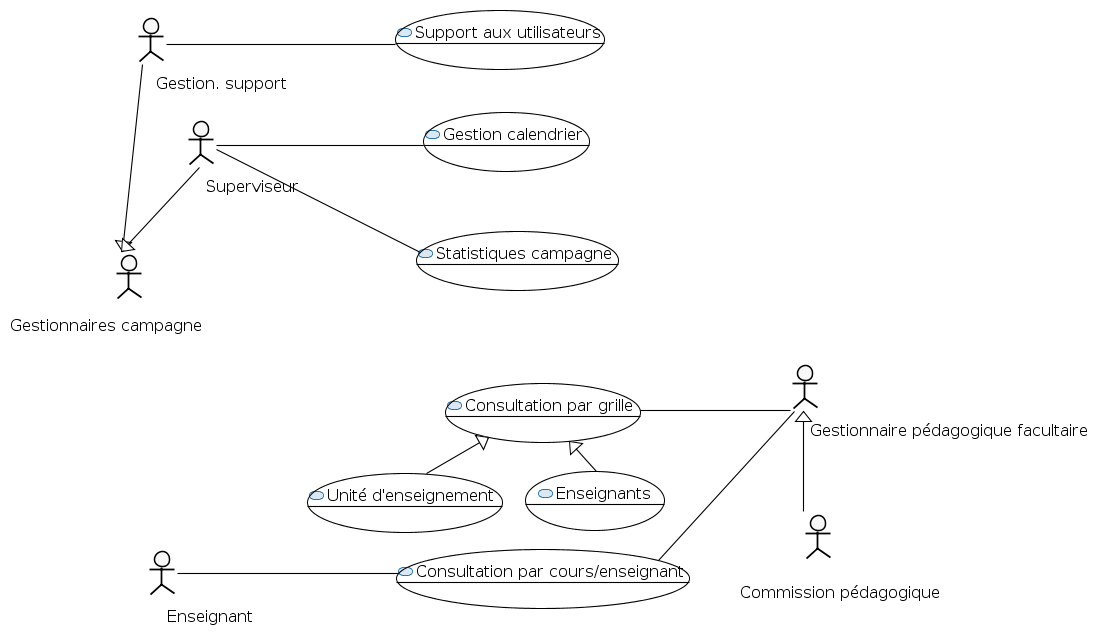
\includegraphics[width=\linewidth]{workspace/evalens-usecases/gestion_campagne.png}
\caption{Diagramme des cas d'utilisation de la gestion de campagne d'évaluation.}
\label{fig:usecase-campagne}
\end{figure}


%%%%%%%%%%%%%%%%%%%%%%%%%%%%%%%%%%%%%%%%%%%%%%%%%%%%%%%%%%%%%%%
%      GESTION DU CALENDRIER
%%%%%%%%%%%%%%%%%%%%%%%%%%%%%%%%%%%%%%%%%%%%%%%%%%%%%%%%%%%%%%%
\subsection{Gestion du calendrier}
La gestion du calendrier est une étape nécessaire à une campagne~; elle permet de définir les périodes de validité de certaines activités ainsi que les dates de planification des tâches, potentiellement par faculté.
Cette gestion permet de déclarer une période de suspension pour toute période définie en cas de besoin.

\noindent Elle est prise en charge par le gestionnaire de campagne.

\noindent Parmi ces dates et périodes, on trouve~:
\begin{itemize}
	\item Invitation à la prise d'avis~: date et heure à laquelle le mail d'invitation à la prise d'avis est envoyé aux étudiants.
	\item Rappel à la prise d'avis~: date et heure à laquelle le mail de rappel de prise d'avis est envoyé aux participants qui n'ont pas rempli certains critères (exemple~: participants ayant répondu à moins de 80~\% des questions).
	\item Prise d'avis~: période durant laquelle les étudiants ont accès aux questionnaires et peuvent les remplir.
	\item Traitement des résultats~: période durant laquelle la commission pédagogique a accès au traitement des résultats. La commission a aussi l'opportunité de consulter les résultats à partir du début de cette période, dès lors que le traitement est terminé.
	\item Consultation des résultats par les enseignants~: date à partir de laquelle les enseignants ont accès aux résultats de la campagne.
	Les enseignants sont notifiés par courriel de cette date par le doyen et le président de commission pédagogique.
	\item Consultation des résultats par grille~: date à partir de laquelle les résultats par grille sont accessibles par un ensemble de rôle.
\end{itemize}
~\newline{}

La constitution du calendrier est régie par les règles et contraintes suivantes~:
\begin{itemize}
	\item Chaque date et période déclarée doit être liée à une campagne.
	\item La période de prise d'avis doit être incluse dans la période de la campagne.
	\item La période de prise d'avis doit durer au moins deux semaines (annexe~\ref{an:regl-cadre}).
	\item La date d'invitation des prises d'avis doit être entérieure à la date de début de la période de prise d'avis.
	\item La date de rappel à la prise d'avis doit être incluse dans la période de prise d'avis.
	\item Le traitement des résultats est suspendu tant qu'une période de prise d'avis est en cours.
	\item La date de consultation des résultats par les enseignants doit être postérieure à la date de fin de la période de traitement des résultats.
\end{itemize}


% \begin{landscape}
\subsubsection{Processus}
\paragraph{Élément déclencheur}~\newline{}

Planification du superviseur pour respecter les décisions du règlement cadre (annexe~\ref{an:regl-cadre}\footnote{Règlement cadre du 02 février 2015 (version 1.1).}).

\paragraph{Planification}\label{sec:calendrier-processus-plan}~\newline{}

\begin{tabularx}{\linewidth}{|X|X|X|} \hline
Fréquence du processus & Début & Fin \\ \hline
Deux fois par année académique (annexe~\ref{an:regl-cadre})~: & & \\
& & \\
Période 2 & En février après la session d'examens de janvier & deux semaines plus tard \\
& & \\ %\hdashline
Périodes 1 et 3 & En juin après la session d'examens de juin & trois semaines plus tard \\
& après la session d'août & deux semaines plus tard \\ \hline
\end{tabularx}
% Info tirées du "règlement cadre" et du cahier des charges.

\paragraph{Data}~\newline{}

\begin{tabularx}{\linewidth}{|X|X|} \hline
Data In & Data Out \\ \hline
N/A & Périodes composant le calendrier de campagne~:
\begin{itemize}
	\item Période de prise d'avis
	\item Date d'invitation à la prise d'avis
	\item Période de traitement des résultats
	\item Date de consultation des résultats
	\item etc.
\end{itemize}
~\\ \hline
\end{tabularx}

% \paragraph{Data In du processus}
% \begin{tabularx}{\linewidth}{|X|X|X|X|} \hline
% Data & Type & Source & Destiné à l'acteur \\ \hline
% \end{tabularx}

\paragraph{Data Out du processus}~\newline{}

\begin{tabularx}{\linewidth}{|X|X|X|X|} \hline
Data & Type & État & Destination \\ \hline
Calendrier & Base de données & Complet, peut faire l'objet de mises à jour & ?? \\ \hline
\end{tabularx}

\paragraph{Acteurs}~\newline{}

\begin{tabularx}{\linewidth}{|X|X|X|X|X|} \hline
Nom & Rôle & Actions & Data In & Data Out \\ \hline
% Commission pédagogique & 
Superviseur & Gestionnaire de calendrier & Établissement des dates & N/A & Calendrier de la campagne \\ \hline
\end{tabularx}

% \end{landscape}

% \begin{chronology}[1]{2016}{2017}{3em}{\linewidth}%
% \event{\decimaldate{15}{02}{2016}}{three}
% \end{chronology}
\begin{figure}[ht]
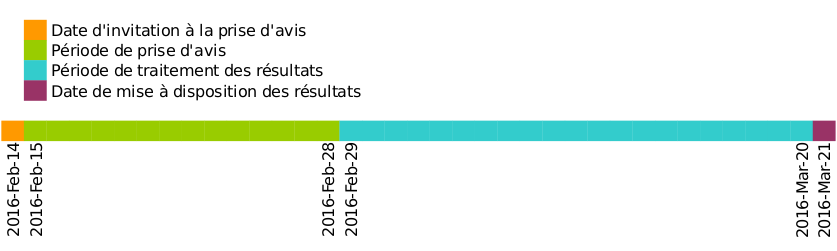
\includegraphics[width=\linewidth]{timeline_exemple.png}
\caption{Exemple de calendrier de campagne d'évaluation.}
\label{fig:calendrier-exemple}
\end{figure}






%%%%%%%%%%%%%%%%%%%%%%%%%%%%%%%%%%%%%%%%%%%%%%%%%%%%%%%%%%%%%%%
%      EXPORTATION
%%%%%%%%%%%%%%%%%%%%%%%%%%%%%%%%%%%%%%%%%%%%%%%%%%%%%%%%%%%%%%%
% \subsection{Exportation}
% Les différentes données accessibles à l'utilisateur doivent pouvoir être exportées en différents formats~:
% \begin{itemize}
% 	\item CSV
% 	\item PDF
% \end{itemize}






%%%%%%%%%%%%%%%%%%%%%%%%%%%%%%%%%%%%%%%%%%%%%%%%%%%%%%%%%%%%%%%
%      STATISTIQUES DE CAMPAGNE
%%%%%%%%%%%%%%%%%%%%%%%%%%%%%%%%%%%%%%%%%%%%%%%%%%%%%%%%%%%%%%%
\subsection{Statistiques de campagne}






%%%%%%%%%%%%%%%%%%%%%%%%%%%%%%%%%%%%%%%%%%%%%%%%%%%%%%%%%%%%%%%
%      SUPPORT UTILISATEURS
%%%%%%%%%%%%%%%%%%%%%%%%%%%%%%%%%%%%%%%%%%%%%%%%%%%%%%%%%%%%%%%
\subsection{Support aux utilisateurs}
























\newpage
\section{Enquête}

\begin{figure}[ht]
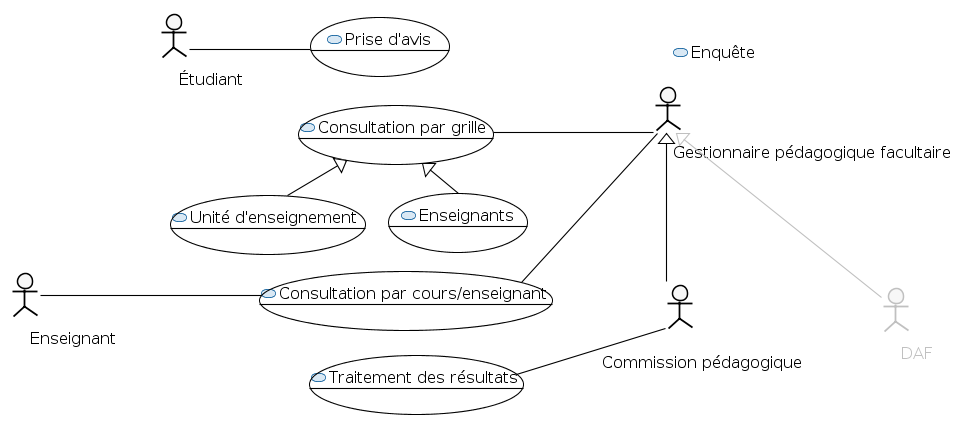
\includegraphics[width=\linewidth]{workspace/evalens-usecases/prise_avis.png}
\caption{Diagramme des cas d'utilisation de la prive d'avis.}
\label{fig:usecase-avis}
\end{figure}

%%%%%%%%%%%%%%%%%%%%%%%%%%%%%%%%%%%%%%%%%%%%%%%%%%%%%%%%%%%%%%%
%      PRISE DES AVIS
%%%%%%%%%%%%%%%%%%%%%%%%%%%%%%%%%%%%%%%%%%%%%%%%%%%%%%%%%%%%%%%
\subsection{Prise des avis}
La prise des avis est le processus dans lequel les étudiants donnent leur avis sur les unités d'enseignement et les enseignants grâce aux questionnaires préalablement approuvés par la CoCoPe et implémentés par le processus de gestion des questionnaires.
%La prise d'avis est essentielle au processus d'évaluation des enseignements~; elle requiert des étudiants qu'ils remplissent les questionnaires d'évaluation concernant les unités d'enseignement qu'ils ont suivies lors de la période couverte par la campagne d'évaluation. % Les étudiants ont donc /l'obligation/ de remplir ces questionnaires.

La prise d'avis est possible uniquement durant la période définie à cet effet dans le calendrier de campagne.
Les étudiants, les unités d'enseignement et les enseignants concernés par la prise d'avis sont ceux déterminés respectivement par le processus de gestion des étudiants, de gestion des unités d'enseignement et des enseignants.

%Les étudiants ont la possibilité de remplir les questionnaires d'évaluation à distance et sont invités à le faire par courriel.
L'étudiant est invité par courriel à participer à la prise d'avis.
Il est alors dirigé vers l'application lui proposant sont programme individuel de cours (PIC) où sont repris les unité d'enseignement faisant partie ou non de la campagne d'évaluation.
Après avoir sélectionné une unité d'enseignement soumise à évaluation, l'étudiant peut choisir les enseignants pour lesquels il donnera sont avis à l'écran suivant qui est constitué du questionnaire d'évaluation.
Une fois le questionnaire rempli, l'étudiant peut le sauvegarder et est redirigé vers son PIC.

Si la prise d'avis est obligatoire, elle est néanmoins anonyme. Le système d'évaluation est capable de déterminer quels étudiants ont rempli les questionnaires, mais pas leurs réponses.

Les réponses entrées par l'étudiant ne sont pas modifiables.

~\footnote{Parler du quorum ici~?}

\subsubsection{Processus}
\paragraph{Élément déclencheur}~\newline{}

Réception de l'invitation à la prise d'avis.

\paragraph{Planification}~\newline{}

La planification de la prise d'avis est asujettie à l'établissement du calendrier de campagne, lui-même définissant une période de prise d'avis au sein de la période de la campagne d'évaluation.

\paragraph{Data}~\newline{}

\begin{tabularx}{\linewidth}{|X|X|} \hline
Data In & Data Out \\ \hline
\begin{itemize}
	\item Questionnaires d'évaluation 
	\item Invitation à la prise d'avis
	\item Rappel à la prise d'avis
\end{itemize}
& Réponses aux questionnaires d'évaluation\\ \hline
\end{tabularx}

\paragraph{Data In du processus}~\newline{}

\begin{tabularx}{\linewidth}{|X|X|X|X|} \hline
Data & Type & Source & Destiné à l'acteur \\ \hline
Questionnaires d'évaluation & Base de données & Commission pédagogique facultaire & Étudiant \\ 
& & & \\
Invitation à la prise d'avis & Courriel & Gestionnaire de communication & Étudiant \\
& & & \\
Rappel à la prise d'avis & Courriel & Gestionnaire de communication & Étudiant \\ \hline
\end{tabularx}

\paragraph{Data Out du processus}~\newline{}

\begin{tabularx}{\linewidth}{|X|X|X|X|} \hline
Data & Type & État & Destination \\ \hline
Réponses aux questionnaires d'évaluation & Base de données & Complet & Commission pédagogique facultaire \\ \hline
\end{tabularx}

\paragraph{Acteurs}~\newline{}

\begin{tabularx}{\linewidth}{|X|X|X|X|X|} \hline
Nom & Rôle & Actions & Data In & Data Out \\ \hline 
Étudiant & Prise d'avis & Répond aux questionnaires d'évaluation & Questionnaires d'évaluation & Réponses aux questionnaires d'évaluation \\ \hline
% À ce niveau, la commission pédagogique facultaire n'est pas un acteur parce qu'elle n'agit pas activement dans le processus de prise d'avis. Elle met à disposition un ensemble de questionnaires et reçoit les réponses sans d'impliquer davantage.
\end{tabularx}






%%%%%%%%%%%%%%%%%%%%%%%%%%%%%%%%%%%%%%%%%%%%%%%%%%%%%%%%%%%%%%%
%      TRAITEMENT DES RÉSULTATS
%%%%%%%%%%%%%%%%%%%%%%%%%%%%%%%%%%%%%%%%%%%%%%%%%%%%%%%%%%%%%%%
\subsection{Traitement des résultats}
La gestion du traitement des résultats concerne l'émission d'une évaluation des unités d'enseignement et des enseignants sur base des résultats de la prise d'avis.
Il permet à la commission pédagogique d'émettre un avis pour chaque unité d'enseignement et chaque enseignant soumis à la campagne d'évaluation.

La période de traitement des résultats est définie dans le calendrier de campagne et débute après la fin de la période de prise d'avis.
À l'issue de la période de prise d'avis, une série de statistiques et d'indicateurs sont mis à disposition de la commission pédagogique afin de les aider à traiter les résultats.
Les indicateurs d'évaluation

Les évaluations émises à l'issue du traitement des résultats sont mises à disposition des gestionnaires pédagogiques facultaires, aux enseignants ainsi qu'aux gestionnaires de campagne.

En cas d'avis potentiellement défavorable, il se passe des choses spéciales (article 9).

Peut être à la base de l'émission d'un avis de circonstance.


\subsubsection{Processus}
\paragraph{Élément déclencheur}~\newline{}

Le traitement des résultats débute à la date définie dans le calendrier de campagne.

\paragraph{Planification}~\newline{}

Le traitement des résultats a lieu à chacune des campagnes d'évaluation.
Ces dernières sont programmées deux fois par an (cf. section~\ref{sec:calendrier-processus-plan}).

\paragraph{Data}~\newline{}

\begin{tabularx}{\linewidth}{|X|X|} \hline
Data In & Data Out \\ \hline
\begin{itemize}
	\item Résultats des prises d'avis
	\item Indicateurs d'évaluation\newline{}
\end{itemize}
 & 
\begin{itemize}
	\item Évaluations des enseignants et des unités d'enseignement
	\item Notification de disponibilité des résultats\footnote{Sans doute à supprimer de cette liste. La notification ne fait partie à proprement parler du processus de traitement des résultats, mais il y fait directement suite. Ne serait-il pas intéressant de le faire apparaître dans le diagramme d'acitivité~?}\newline{}
\end{itemize}
\\ \hline
\end{tabularx}

\paragraph{Data In du processus}~\newline{}

\begin{tabularx}{\linewidth}{|X|X|X|X|} \hline
Data & Type & Source & Destiné à l'acteur \\ \hline
Résultats des prises d'avis & Base de données & Prise d'avis des étudiants & Commission pédagogique \\
Indicateurs d'évaluation & Base de données & Calculs statistiques & Commission pédagogique \\ \hline
\end{tabularx}

\paragraph{Data Out du processus}~\newline{}

\begin{tabularx}{\linewidth}{|X|X|X|X|} \hline
Data & Type & État & Destination \\ \hline
Évaluations des enseignants et des unités d'enseignement & ??\footnote{On donne accès à un pan de l'application. À quel type cela correspond-il ?} & ?? & 
\begin{itemize}
	\item Enseignants
	\item Gestionnaires de campagne
	\item Gestionnaires pédagogiques faculaires\newline{}
\end{itemize}
\\
Notification de disponibilité des résultats & Courriel & Complet & Enseignants \\ \hline
\end{tabularx}

\paragraph{Acteurs}~\newline{}

\begin{tabularx}{\linewidth}{|X|X|X|X|X|} \hline
Nom & Rôle & Actions & Data In & Data Out \\ \hline 
Commission pédagogique & Traitement des résultats & Sur base des prises d'avis, décide d'une évaluation pour l'enseignant et l'unité d'enseignement concernés & Prises d'avis & Évaluations \\ \hline
\end{tabularx}






%%%%%%%%%%%%%%%%%%%%%%%%%%%%%%%%%%%%%%%%%%%%%%%%%%%%%%%%%%%%%%%
%      CONSULTATION DES RÉSULTATS PAR GRILLES
%%%%%%%%%%%%%%%%%%%%%%%%%%%%%%%%%%%%%%%%%%%%%%%%%%%%%%%%%%%%%%%
\subsection{Consultation des résultats par grille}
La consultation des résultats par grille reprend toutes les unités d'enseignement  d'une campagne ainsi que les enseignants associés.\footnote{Lorsqu'un gestionnaire pédagogique effectute une consultation par grille, voit-il toutes les UE de la campagne d'évaluation, ou uniquement celle rattachée à sa faculté~?}\footnote{Le superviseur a aussi accès à cette consultation, et lui voit tout le monde. Ne devrait-on pas l'ajouter comme acteur~?}
Cette consultation est accessible aux gestionnaires pédagogiques faculaires dès l'ouverture de la période de traitement des résultats.

Lors de l'affichage des résultats, les informations reprises sont les suivantes~:
\begin{itemize}
	\item Unité d'enseignement
	\item Titulaire
	\item Nombre d'étudiants inscrits
	\item Quorum
	\item Indicateur d'évaluation ou l'évaluation émis par la commission pédagogique si elle l'a déjà encodée
	\item ...
\end{itemize}
~\\

Les résultats peuvent aussi être filtré suivant les paramètres suivants~:
\begin{itemize}
	\item Enseignant
	\item Unité d'enseignement
	\item Faculté d'appartenance de l'unité d'enseignement
	\item Statut de l'évaluation~: émise ou non
	\item Évaluation~: au-dessus ou en dessous d'un certain seuil
	\item ...
\end{itemize}

\subsubsection{Processus}
\paragraph{Élément déclencheur}~\newline{}

Ouverture de la période de traitement des résultats à la date définie dans le calendrier de campagne.

\paragraph{Planification}~\newline{}

L'ouverture de la consultation des résultats a lieu une fois par campagne d'évaluation.
Cette consultation n'a ensuite pas de date de cloture.

\paragraph{Data}~\newline{}

\begin{tabularx}{\linewidth}{|X|X|} \hline
Data In & Data Out \\ \hline
\begin{itemize}
	\item Résultats de la prise d'avis
	\item Évaluations des enseignements émises par la commission pédagogique \newline{}
\end{itemize}
& N/A \\ \hline
\end{tabularx}

\paragraph{Data In du processus}~\newline{}

\begin{tabularx}{\linewidth}{|X|X|X|X|} \hline
Data & Type & Source & Destiné à l'acteur \\ \hline
Résultats de la prise d'avis & Base de données & Prise d'avis & Gestionnaire pédagogique facultaire \\
Évaluations des enseignements & Base de données & Commission pédagogique & Gestionnaire pédagogique facultaire \\ \hline
\end{tabularx}

% \paragraph{Data Out du processus}~\newline{}

% \begin{tabularx}{\linewidth}{|X|X|X|X|} \hline
% Data & Type & État & Destination \\ \hline
%  &  &  &  \\ \hline
% \end{tabularx}

\paragraph{Acteurs}~\newline{}

\begin{tabularx}{\linewidth}{|X|X|X|X|X|} \hline
Nom & Rôle & Actions & Data In & Data Out \\ \hline 
Gestionnaire pédagogique facultaire & Consultation des résultats par grille & Consulte les résultats des prises d'avis et les évaluations sous forme de grille. Peut filtrer les résultats.\footnote{Bof, pas vraiment une action, ce n'est qu'une manipulation de la vue.} & Résultats et évaluations & N/A \\ \hline
\end{tabularx}






%%%%%%%%%%%%%%%%%%%%%%%%%%%%%%%%%%%%%%%%%%%%%%%%%%%%%%%%%%%%%%%
%      CONSULTATION PAR COURS/ENSEIGNANT
%%%%%%%%%%%%%%%%%%%%%%%%%%%%%%%%%%%%%%%%%%%%%%%%%%%%%%%%%%%%%%%
\subsection{Consultation par unité d'enseignement/enseignant}

La consultation de résultats par unité d'enseignement ou par enseignant reprend respectivement les évaluations d'une seule unité d'enseignement et des enseignants associés ou les résultats d'un enseignant et des unités d'enseignement dans lesquelles il est impliqué.

Ces évaluations sont émises par la commission pédagogique durant la période de traitement des résultats et les enseignants sont notifiés de leur disponibilité par le doyen et le président de la commission pédagogique.

Les évaluations sont consultables par les enseignants concernés ainsi que par les gestionnaires pédagogiques faculaires.

Les enseignants ont la possibilité de consulter leurs évaluations de deux façons différentes~:
\begin{itemize}
	\item en vue globale rassemblant toutes leurs unités d'enseignement~;
	\item une unité d'enseignement à la fois.
\end{itemize}

Si l'enseignant est titulaire de l'unité d'enseignement, il a accès aux évaluations des enseignants non-titulaires associés en plus des siennes.

% Les titulaires des unités d'enseignement peuvent consulter
Dès lors que les résultats d'évaluation sont consultables, ils le restent indéfiniment.

\subsubsection{Processus}
\paragraph{Élément déclencheur}~\newline{}

Annonce de la disponibilité des résultats par le doyen et le président de la commission pédagogique.

\paragraph{Planification}~\newline{}

Programmée à chaque campagne d'évaluation, après la période de traitement des données, à une date définie dans le calendrier de campagne.

\paragraph{Data}~\newline{}

\begin{tabularx}{\linewidth}{|X|X|} \hline
Data In & Data Out \\ \hline
Évaluation des enseignements & N/A \\ \hline
\end{tabularx}

\paragraph{Data In du processus}~\newline{}

\begin{tabularx}{\linewidth}{|X|X|X|X|} \hline
Data & Type & Source & Destiné à l'acteur \\ \hline
Évaluation des enseignements & Base de données & Commission pédagogique &
\begin{itemize}
	\item Enseignants
	\item Gestionnaires pédagogiques facultaires\newline{}
\end{itemize}
\\ \hline
\end{tabularx}

% \paragraph{Data Out du processus}~\newline{}

% \begin{tabularx}{\linewidth}{|X|X|X|X|} \hline
% Data & Type & État & Destination \\ \hline
%  &  &  &  \\ \hline
% \end{tabularx}

\paragraph{Acteurs}~\newline{}

\begin{tabularx}{\linewidth}{|X|X|X|X|X|} \hline
Nom & Rôle & Actions & Data In & Data Out \\ \hline 
\begin{itemize}
	\item Enseignant
	\item Gestionnaire pédagogique facultaire
\end{itemize}
& Consultation des évaluations & Consulte les évaluations émises par la commission pédagogique, un enseignant ou une unité d'enseignement à la fois. & Évaluations & N/A \\ \hline
\end{tabularx}




\appendix
\renewcommand{\partname}{Annexe}
\setcounter{part}{0}%Reset counter
\part{Règlement cadre}\label{an:regl-cadre}

\includepdf[pages={-}]{annexes/Reglement-cadre_Evaluation_Enseignements_v1_1.pdf}

\part{Cahier des charges}

\includepdf[pages={-}]{annexes/evalens-application-cahier-charges.pdf}

\end{document}


% \begin{landscape}
% \subsubsection{Processus}
% \paragraph{Élément déclencheur}~\newline{}

% \paragraph{Planification}~\newline{}

% \begin{tabularx}{\linewidth}{|X|X|X|} \hline
% Fréquence du processus & Début & Fin \\ \hline
% &  &  \\ \hline
% \end{tabularx}

% \paragraph{Data}~\newline{}

% \begin{tabularx}{\linewidth}{|X|X|} \hline
% Data In & Data Out \\ \hline
%  & \\ \hline
% \end{tabularx}

% \paragraph{Data In du processus}~\newline{}
% 
% \begin{tabularx}{\linewidth}{|X|X|X|X|} \hline
% Data & Type & Source & Destiné à l'acteur \\ \hline
% \end{tabularx}

% \paragraph{Data Out du processus}~\newline{}

% \begin{tabularx}{\linewidth}{|X|X|X|X|} \hline
% Data & Type & État & Destination \\ \hline
%  &  &  &  \\ \hline
% \end{tabularx}

% \paragraph{Acteurs}~\newline{}

% \begin{tabularx}{\linewidth}{|X|X|X|X|X|} \hline
% Nom & Rôle & Actions & Data In & Data Out \\ \hline 
% & &  &  &  \\ \hline
% \end{tabularx}

% \end{landscape}